\documentclass[10pt,a4paper]{book}
\usepackage[utf8]{inputenc}
\usepackage{amsmath}
\usepackage{amsfonts}
\usepackage{amssymb}
\usepackage{minted}
\usepackage{xcolor}
\usepackage{graphicx}
\definecolor{mygray}{gray}{0.9}
\title{Programming personal reference\\ \Large Concepts in a nutshell}
\author{Nicolò Fornari}
\begin{document}
\maketitle
\chapter{OOP}
\section{Inheritance}
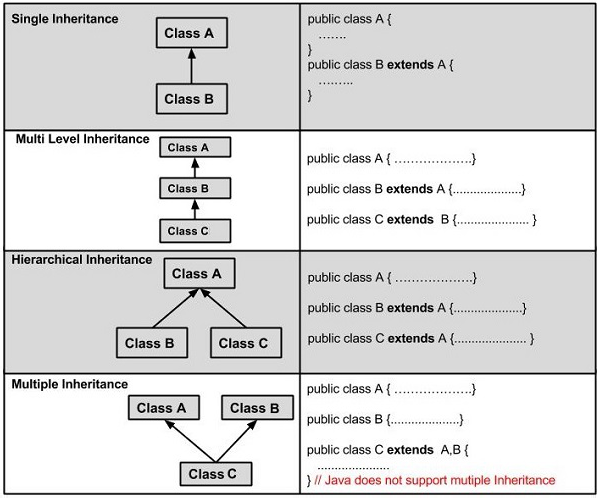
\includegraphics[scale=0.7]{img/inheritance.jpg}
\newline
Così come per scope considero la variabile più prossima, per le classi cerco il metodo più prossimo.\\\\
In realtà ogni classe che sembra non ereditare niente eredità da Object.\\
La classe Object è la root di tutta la gerarchia di classi.\\\\
Se voglio usare un metodo della superclasse: super.metodo()\\
Si può iterare: super.super.metodo()
\newpage
\textbf{Esempio}\\
\begin{minted}[
bgcolor=mygray,
]{java}
public class MySlider extends javafx.scene.control.Slider {
    
    public MySlider() {
        super(0,255,0);
    
        setShowTickLabels(true);
        setShowTickMarks(true);
        setMajorTickUnit(50);
        setMinorTickCount(5);
        setBlockIncrement(10);
    }
}
\end{minted}
\newpage

\section{Polimorphism}
Voglio creare a runtime (Dynamic Binding) oggetti diversi a seconda delle scelte dell'utente\\\\
\begin{minted}[
bgcolor=mygray,
]{java}
public class Main {
    public static void main(String[] args) {
        Stack s;
        if (args[0] != "")
            s=new Coda();
        else
            s = new Pila();
        s.inserisci(1);
        s.inserisci(2);
        s.inserisci(3);
        for (int k=0;k<=4;k++){
            int v=s.estrai();
            System.out.println(v);
        }
    }

\end{minted}
\newpage
\section{Abstraction}
Non possono essere istanziate,devono essere subclassate.\\\\
\begin{minted}[
bgcolor=mygray,
]{java}
import java.util.*;
public abstract class Stack extends LinkedList {
    public void inserisci(int x) {
    Number n = new Number(x);
    this.add(n);
    }

    abstract public int estrai();
}

\end{minted}
\\\\
\begin{minted}[
bgcolor=mygray,
]{java}
import java.util.*;

class Pila extends Stack {
    @Override
    public int estrai() {
        Number x = null;
        Iterator iter = this.iterator();
        while (iter.hasNext()) {
            x = (Number) iter.next();
        }
        if (x == null) {
            System.out.println("Pila vuota");
            System.exit(1);
        }
        iter.remove();
        return x.getInt();
    }
}

\end{minted}
\newpage
\section{Encapsulation}
Encapsulation in Java is a mechanism of wrapping the data (variables) and code acting on the data (methods) together as a single unit. In encapsulation, the variables of a class will be hidden from other classes, and can be accessed only through the methods of their current class (called setter and getter).\\\\
\textbf{Implementation:}
\begin{itemize}
\item Declare the variables of a class as private.
\item Provide public setter and getter methods to modify and view the variables values
\end{itemize} 
\textbf{Benefits}
\begin{itemize}
\item The fields of a class can be made read-only or write-only.
\item A class can have total control over what is stored in its fields.
\item The users of a class do not know how the class stores its data. A class can change the data type of a field and users of the class do not need to change any of their code.
\end{itemize}
\newpage
\section{Interfaces}
\begin{tabular}{|c|c|}
\hline 
Interface & Abstract class \\ 
\hline 
Solo metodi non implementati & Può avere metodi implementati e variabili.\\
Non può contenere variabili & -\\
Una classe può implementare più interfacce alla volta. & Non vale l'ereditarietà multipla\\
\hline 
\end{tabular} 
\\\\
Non è possibile che una classe erediti da due classi astratte contemporaneamente, perché se viene chiamato un metodo non sovrascritto dalla sottoclasse ed implementato in entrambe le superclassi astratte, ci sarebbe l'abiguità di andare a pescare da una superclasse piuttosto che dall'altra.
\\\\
\begin{minted}[
bgcolor=mygray,
]{java}
public class drawCircle implements EventHandler {

    Color color;
    Canvas canv;
    int r = 50;
    
    public drawCircle(Color color,Canvas canv) {
        this.color = color;
        this.canv = canv;
    }
    
    @Override
    public void handle(Event t) {
        double w = canv.getWidth();
        double h = canv.getHeight();
        
        int x = (int) (Math.random()*w);
        int y = (int) (Math.random()*h);
        
        canv.getGraphicsContext2D().setFill(color);
        canv.getGraphicsContext2D().fillOval(x,y,r,r);
    }
} 

\end{minted}
\newpage
\section{Packages}
Packages in Java are used to control access, making usage of classes and interfaces easier and to prevent naming conflicts.\\
It is a good practice to define your own package: in this way it is easy to determine which classes and interfaces are related.\\
Since the package creates a new namespace there won't be any name conflicts with names in other packages. 
\newpage
\section{Modifiers}
\textbf{Access modifiers}
\begin{itemize}
\item (default) visible to the package
\item private: visible to the class only
\item protected: visible to the package and all subclasses
\item public: visible to the world
\end{itemize}
\textbf{Non access}
\begin{itemize}
\item static\\
Variables and methods associated to a class rather than to an object are static. Static variables are used as shared variables among instances.\\
Static methods can be called without any instance of the class.
\item final
\begin{enumerate}
\item final variables are constant
\item final methods can not be overwritten
\item final classes can not be subclassed
\end{enumerate}
\item abstract
\begin{enumerate}
\item abstract classes must be subclassed and can not be instantiated
\item abstract methods must be overwritten
\end{enumerate}
\end{itemize}
\newpage
\section{Collections}
Una collection è un oggetto che raggruppa elementi multipli in un'unica entità, all' interno di cui i dati possono essere trattati o trasferiti da un metodo ad un altro.\\\\
\begin{tabular}{|c|c|c|c|}
\hline 
- & Presenza di duplicati  & Accessibile  & Ordine di inserimento\\
- & (come identificatore) & con un indice & mantenuto \\
\hline 
Set & No & No & No \\ 
\hline 
List & Si & Si & Si \\ 
\hline 
\end{tabular} 
\\\\
Poichè una Collection prende in input degli Oggetti, se voglio creare una Collection di variabili primitive (eg interi) ho bisogno di un wrapper per la variabile (eg. Integer)\\\\
\begin{minted}[
bgcolor=mygray,
]{java}
public class Mazzo {
    
    List<Carta> Deck;
    int[] valori = {1,2,3,4,5,6,7,8,9,10};
    String[] semi = {"Denari","Spade","Bastoni","Coppe"};
    
    public Mazzo() {
        Deck = new ArrayList<>();
        for (int i=0;i<4;i++) {
                for (int j=0;j<10;j++) {
                    Carta newCard = new Carta(semi[i],valori[j]);
                    Deck.add(newCard);
                    
                }
        }
        Collections.shuffle(Deck);
    }
}

\end{minted}
\\\\
The Collections class provides three constants, representing the empty Set, the empty List, and the 
empty Map 
\begin{itemize}
\item $Collections.EMPTY\_SET $
\item $Collections.EMPTY\_LIST $
\item $Collections.EMPTY\_MAP $
\end{itemize}
The main use of these constants is as input to methods that take a Collection of values, when you 
don't want to provide any values at all. 

\newpage
\section{Object ordering - comparable}
A List l may be sorted as follows: \\
Collections.sort(l); \\\\
If the list consists of String elements, it will be sorted into lexicographic (alphabetical) order. \\
If it consists of Date elements, it will be sorted into chronological order. \\
How does Java know how to do this? \\
String and Date both implement the Comparable interface. The Comparable interfaces provides a natural ordering for a class, which allows objects of that class to be sorted automatically. \\\\
int compareTo(Object o) \\\\
Compares this object with the specified object for order. Returns a negative integer, zero, or a positive integer as this object is less than, equal to, or greater than the specified object. 
\\\\
\begin{minted}[
bgcolor=mygray,
]{java}
public class Carta implements Comparable { 
    String seme;
    String t;
    int valore;
    
    public Carta(String seme, int valore) {
        this.seme = seme;
        this.valore = valore;
    }
    
    @Override
    public int compareTo(Object o) {
        Carta c = (Carta) o;
        return this.valore-c.valore;
    }

\end{minted}

\newpage
\section{Object ordering - comparator}

\begin{minted}[
bgcolor=mygray,
]{java}
public class Giocatore {
    List<Carta> Mano;
    
    public Giocatore() {
        Mano = new ArrayList();
    }

    public void sortHandByValue() {
        Comparator cmp1 = new ComparatorByValue();
        Collections.sort(Mano,cmp1);
    }
    
    public void sortHandBySeed() {
        Comparator cmp2 = new ComparatorBySeed();
        Collections.sort(Mano,cmp2);
    }
}

\end{minted}
\\\\
\begin{minted}[
bgcolor=mygray,
]{java}
public class ComparatorBySeed implements Comparator {
    
    @Override
    public int compare(Object o1,Object o2) {
        Carta c1 = (Carta) o1;
        Carta c2 = (Carta) o2;
        return c1.seme.compareTo(c2.seme);
    }
}

\end{minted}
\\\\
\begin{minted}[
bgcolor=mygray,
]{java}
public class ComparatorByValue implements Comparator {
    
    @Override
    public int compare(Object o1,Object o2) {
        Carta c1 = (Carta) o1;
        Carta c2 = (Carta) o2;
        return c1.valore - c2.valore;
    } 

\end{minted}
\newpage
\section{Listener}
\textbf{Listener esterno}\\\\
\begin{minted}[
bgcolor=mygray,
]{java}
Listener lsn = new Listener(this);
sp.addEventHandler(MouseEvent.MOUSE_CLICKED, lsn);

\end{minted}
\\\\
\begin{minted}[
bgcolor=mygray,
]{java}
public class Listener implements EventHandler {
    SimEsame w = null;
     
    Listener(SimEsame w) {
        this.w = w;
    }
    
    @Override
    public void handle(Event t) {
        w.addCross();
        int id = Integer.parseInt(((Circle)t.getTarget()).getId());
    }
}

\end{minted}
\\\\
\textbf{Listener interno}\\\\
\begin{minted}[
bgcolor=mygray,
]{java}
Button btn = new Button();
btn.setText("Reset");
Reset reset  = new Reset();
btn.addEventHandler(ActionEvent.ACTION, reset);



class Reset implements EventHandler {
        @Override
        public void handle(Event t) {
            updateScore();
                
            }
        }
    }

\end{minted}
\\\\
\textbf{Listener anonimo}\\\\
\begin{minted}[
bgcolor=mygray,
]{java}
Circle c = new Circle(r*i);
c.setOnMouseClicked(new EventHandler<MouseEvent>() {
                @Override public void handle(MouseEvent event) {
                x = event.getX();
                y = event.getY();
        }
    });

\end{minted}
\newpage
\textbf{Self listener}\\\\
\begin{minted}[
bgcolor=mygray,
]{java}
public class SelfListener extends Application implements EventHandler {
    
    @Override
    public void start(Stage primaryStage) {
        Button btn = new Button();
        btn.setText("Say 'Hello World'");
        btn.addEventHandler(ActionEvent.ACTION, this);

        StackPane root = new StackPane();
        root.getChildren().add(btn);
        
        Scene scene = new Scene(root, 300, 250);
        
        primaryStage.setTitle("Hello World!");
        primaryStage.setScene(scene);
        primaryStage.show();
    }

    public static void main(String[] args) {
        launch(args);
    }

    @Override
    public void handle(Event event) {
        System.out.println("Hi");
    }

\end{minted}
\newpage
\section{Best practices}
\begin{itemize}
\item {\bf Read code}\\
It is impossible to become a good writer without having read books written by others.
\item \textbf{Documentation}
\item \textbf{Follow the defined standards}\\
File, functions and variable naming conventions, list of do's and don'ts, history, indentation, comments.
\item \textbf{Code should be written to be reviewed}\\
Self review to avoid
\begin{enumerate}
\item Not following standards
\item Not keeping performance in mind
\item History, indentation, comments not appropriate
\item Poor readability
\item Open files not closed
\item Allocated memory not released
\item Too much hard coding
\item Too many global variables
\item Poor error handling
\item No modularity
\item Repeated code
\end{enumerate}
\item \textbf{Testing} is mandatory after every small or big change
\item \textbf{Keep code safe} with code versioning software
\item \textbf{Tools and techniques handy}
\end{itemize}

\textbf{Principio di Parna} il committente di una funzione deve dare all'implementatore tutte le informazioni necessarie a realizzare la funzione e nulla di più.
\chapter{Data structures}
\section*{Classification}
\begin{itemize}
\item \textbf{Linear:} data are in sequence
\item \textbf{Non Linear}
\item \textbf{Static:} the number of elements remains constant
\item \textbf{Dynamic:} the number of elements can change in time
\item \textbf{Homogeneous:} elements of the same type
\item \textbf{Non homogenenous}
\end{itemize}
\section{Sequence}
Dynamic and linear, possibly containing duplicates. To access a generic item it is necessary to scan the entire sequence either from the beginning or from the end.
\section{Set}
Collection of different elements (no duplicates are allowed). Elements do not have a position.
\section{Dictionary}
It is a key-value map.\\
\textbf{Example:} P2P systems use a DHT (distribute hash table).
\section{Trees and graphs}
\textbf{Example:} the base structure of a file system is a tree. Directories are the vertices while files are the leaves. Since some file systems allow to list the same file in multiple directories by the means of symbolic links, such file systems are DAG (directed acyclic graphs).
\section{Stack and queues}
\section{Queues with priority and disjoint sets}
\chapter{Programming techniques}
\section{Divide et impera}
\section{Dynamic programming}
\section{Greedy}
\section{Backtrack}
\end{document}